\documentclass[9pt]{beamer}
\usepackage[utf8]{inputenc}
\usepackage[T1]{fontenc}
\usepackage{lmodern}
\usepackage[polish]{babel}
\usepackage{amsmath}
\usepackage{graphicx}
\usetheme{metropolis}

\title{A11 — Dyfuzja innowacji i popytu na rynku}
\author{Wojciech Bartoszek \ Łukasz Checiak}
\date{}

\begin{document}

\begin{frame}
  \titlepage
\end{frame}

% --- Zadanie 1 ---
\begin{frame}{Zadanie 1 — Model i kontekst}
\vspace{-0.5em}
\begin{itemize}
  \item Model: $u_t = D\Delta u + (p+q u)(1-u)$ — łączenie Bassa i F-KPP.
  \item Interpretacja: $p$ = innowacja (zew.), $q$ = imitacja (wewn.), $D$ = dyfuzja (przestrz.).
  \item Kluczowy insight: krzywa adopcji typu S; przestrzenne modele dają propagujące się fale.
\end{itemize}
\end{frame}

% --- Zadanie 2 ---
\begin{frame}{Zadanie 2 — Porównanie solverów}
\begin{columns}
\begin{column}{0.55\textwidth}
\vspace{-0.5em}
\begin{itemize}
  \item Testowane solvery: explicit, semi-implicit, Crank–Nicolson.
  \item Czas (średnio): explicit ~0.0048 s; semi-implicit ~0.0329 s; CN ~0.0350 s.
  \item Wniosek: explicit najszybszy dla małych testów, ale wymaga małych \(\Delta t\) (CFL).
\end{itemize}
\end{column}
\begin{column}{0.45\textwidth}
  \centering
  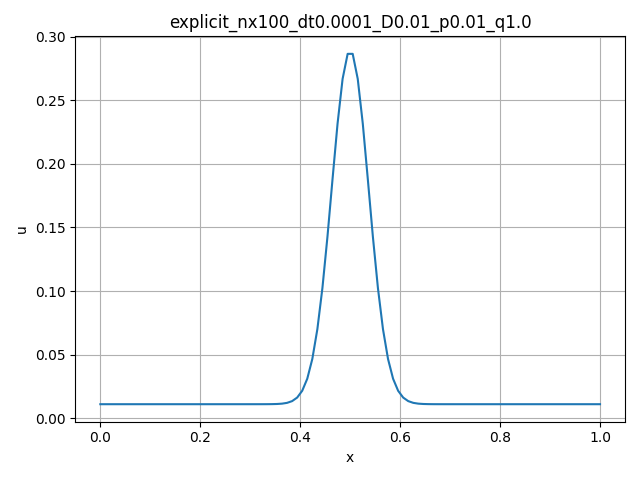
\includegraphics[width=\textwidth]{../zad2/results/explicit_nx100_dt0.0001_D0.01_p0.01_q1.0.png}
  \par\bigskip\centering\scriptsize\textit{Przykładowy profil $u(x)$ (explicit)}
\end{column}
\end{columns}
\end{frame}

% --- Zadanie 3 ---
\begin{frame}{Zadanie 3 — Surogat ODE i NN}
\begin{itemize}
  \item Uśrednienie PDE dało ODE: $\dot U=(p+qU)(1-U)$ — szybkie przybliżenie średniej.
  \item NN (MLP) jako surogat: wejście $(t,D,p,q) \mapsto U(t)$ — natychmiastowa predykcja.
  \item Czas inferencji: ODE ~1.29 ms, NN ~0.87 ms; dobry kompromis dokładność/prędkość.
\end{itemize}
\vspace{0.6em}
\centering
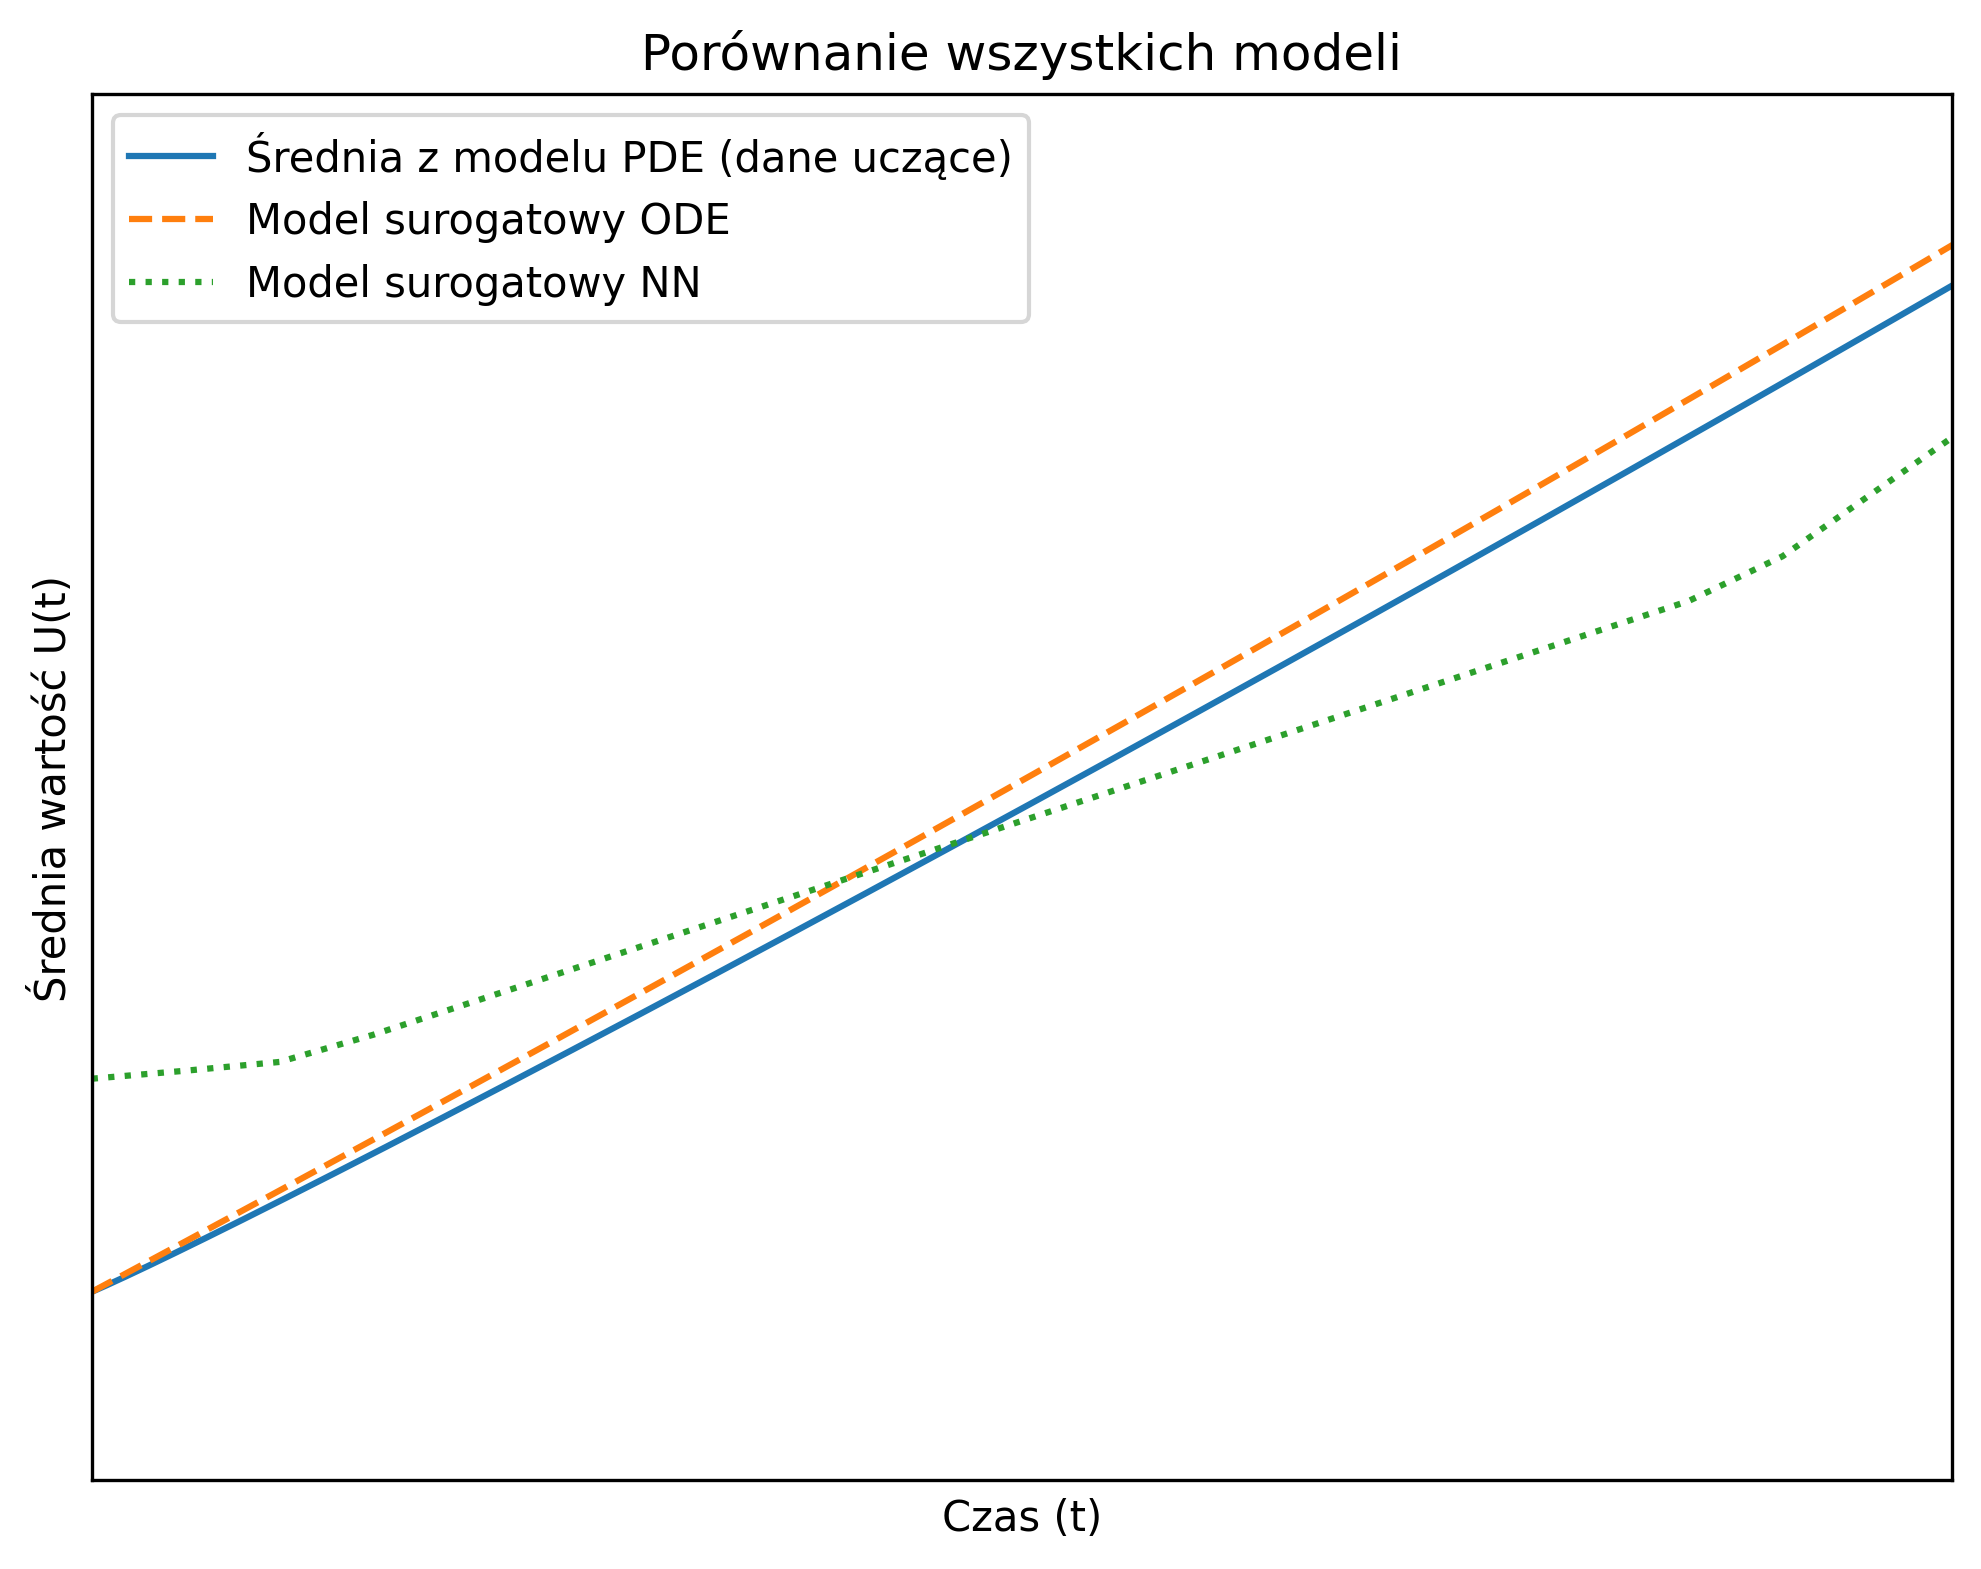
\includegraphics[width=0.7\textwidth]{../presentation/comparison_plot.png}
\end{frame}

% --- Zadanie 4 ---
\begin{frame}{Zadanie 4 — Analiza wrażliwości}
\begin{itemize}
  \item Metody: Morris (screening) i Sobol (wariancja globalna).
  \item Wynik: parametr \textbf{q} (imitacja) ma dominujący wpływ (wysokie $\mu^*$ i $S_T$); $p$ umiarkowane, $D$ mały wpływ na średnią.
\end{itemize}
\vspace{0.6em}
\centering
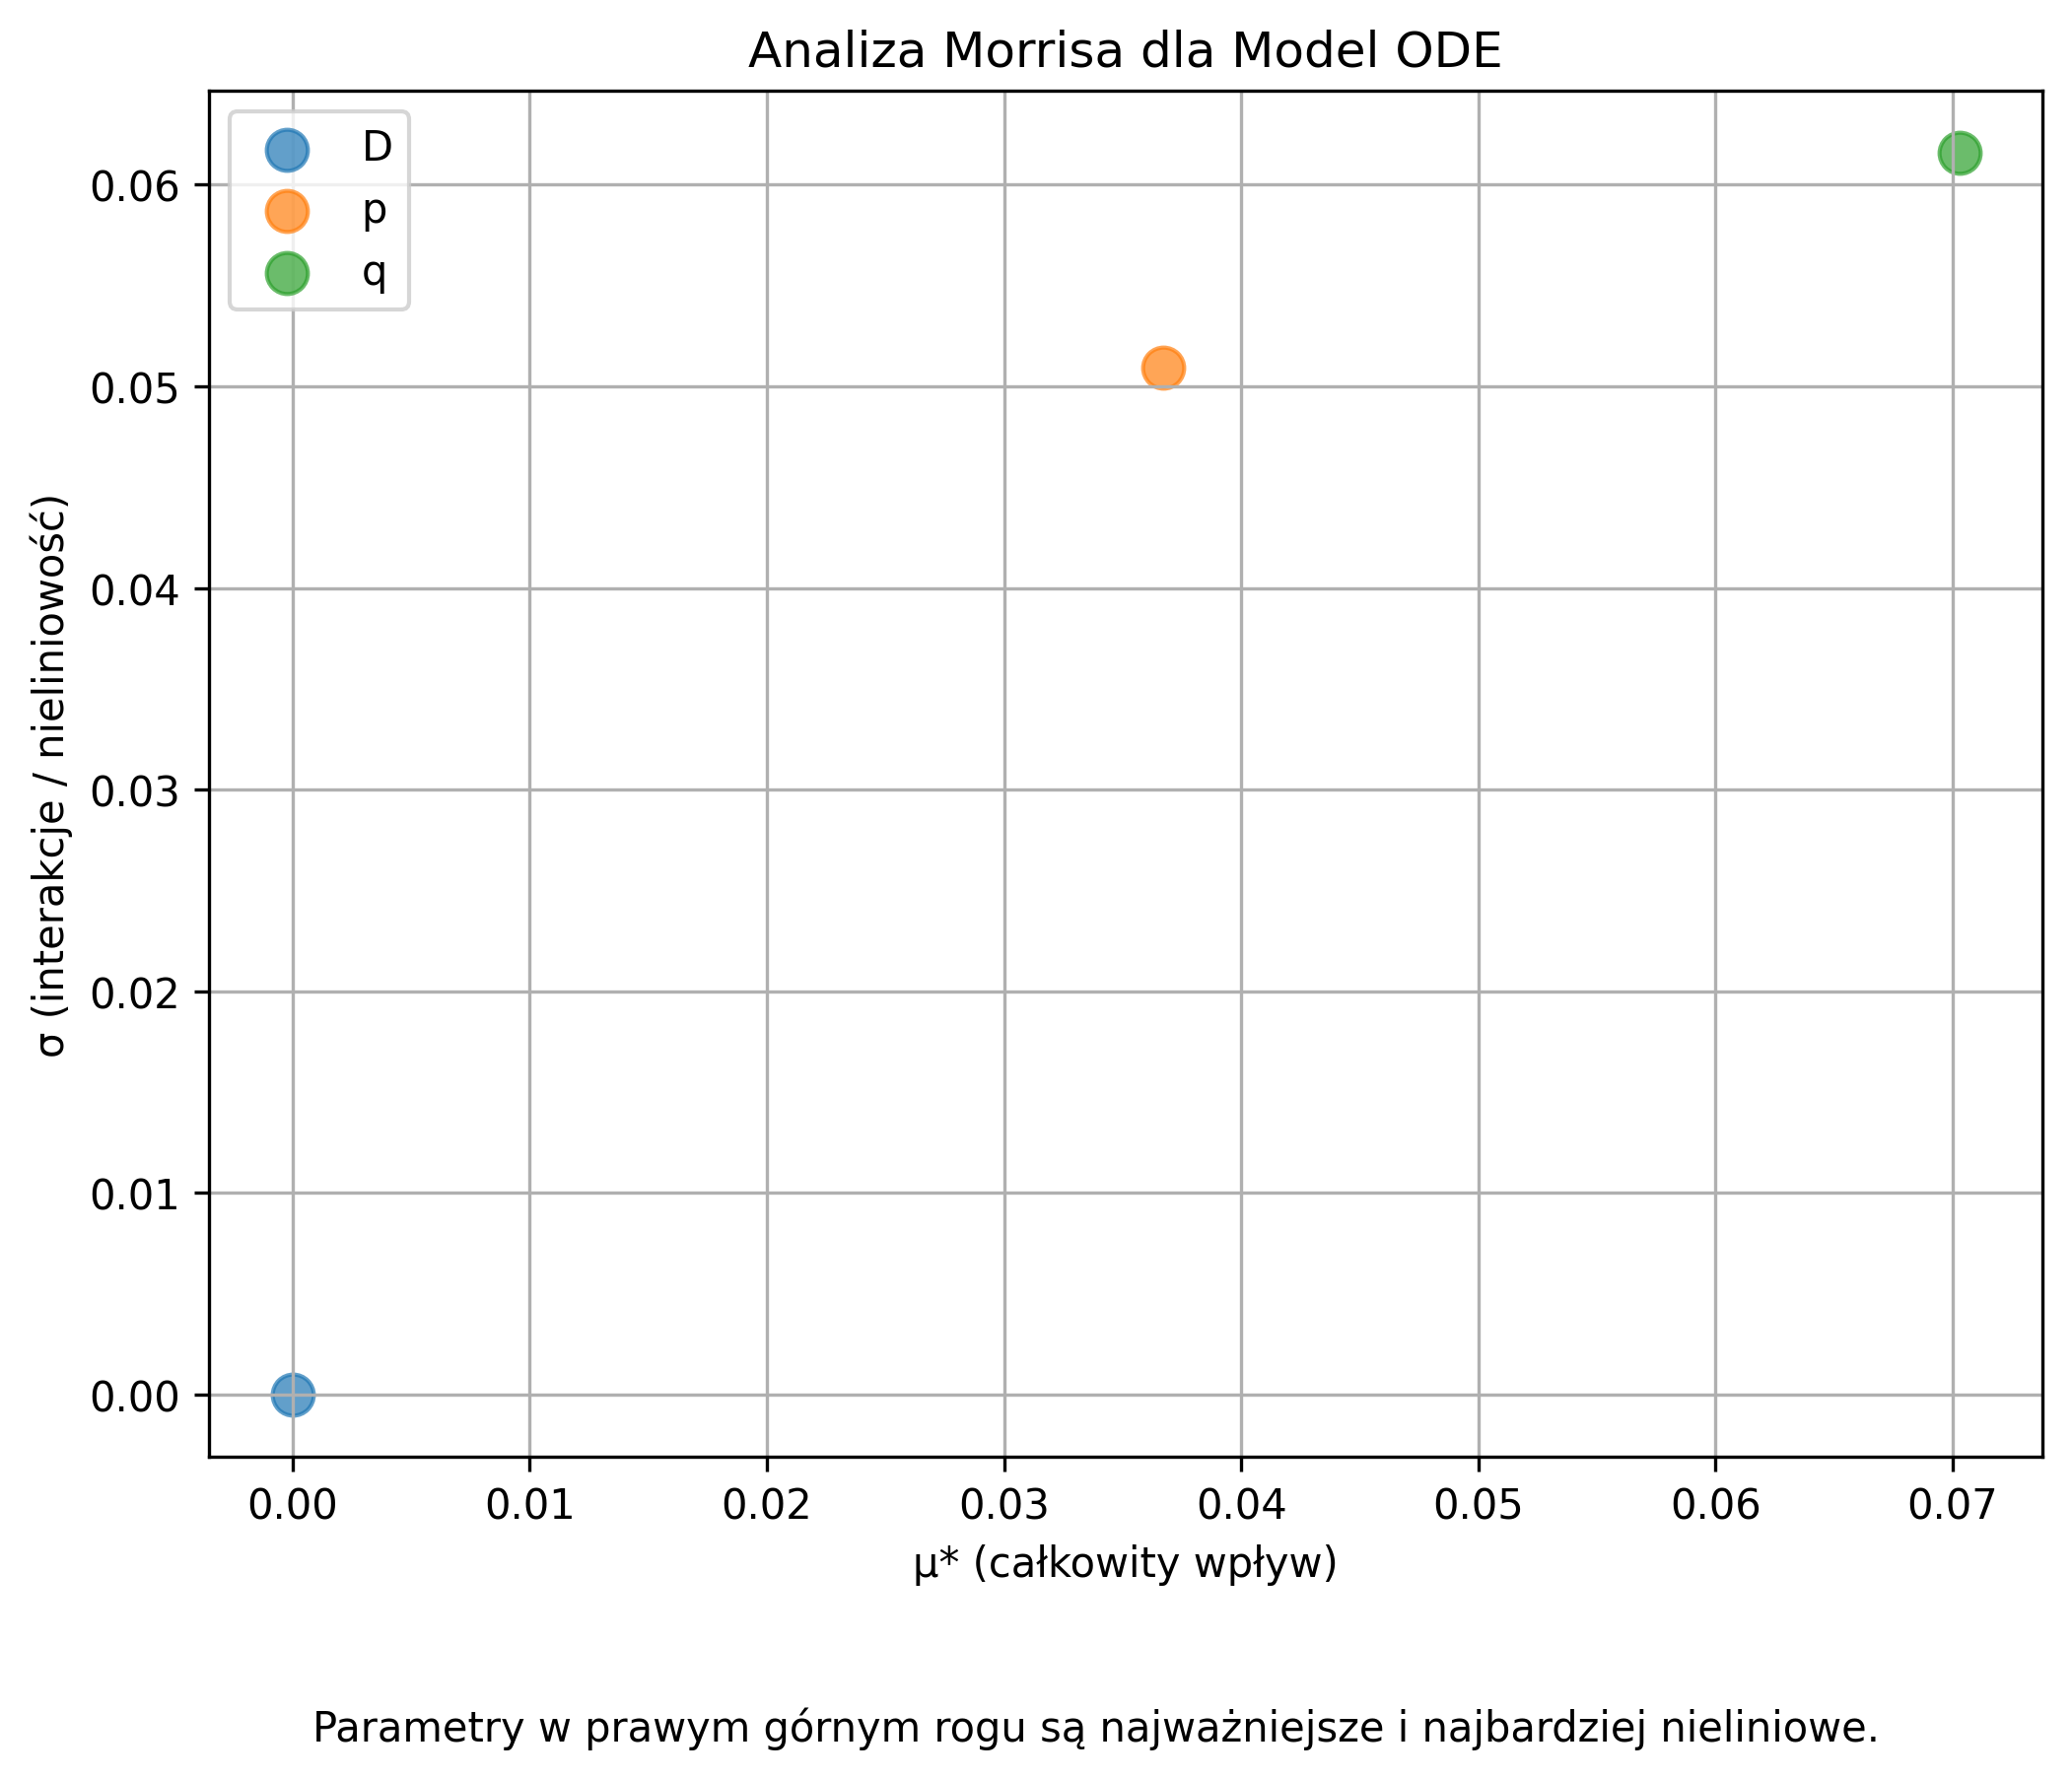
\includegraphics[width=0.6\textwidth]{../presentation/figures/morris_model_ode.png}
\end{frame}

% --- Zadanie 5 ---
\begin{frame}{Zadanie 5 — Asymilacja danych}
\begin{itemize}
  \item Cel: Estymacja parametrów + stanu na podstawie zaszumionych obserwacji.
  \item ODE: 3D-Var szybki i najlepszy (RMSE ~0.0061). ABC wolniejszy, RMSE ~0.0117.
  \item PDE: ABC radzi sobie lepiej (RMSE ~0.026) niż przerwana 3D-Var (RMSE ~0.248) przy limitowanym budżecie.
\end{itemize}
\vspace{0.6em}
\centering
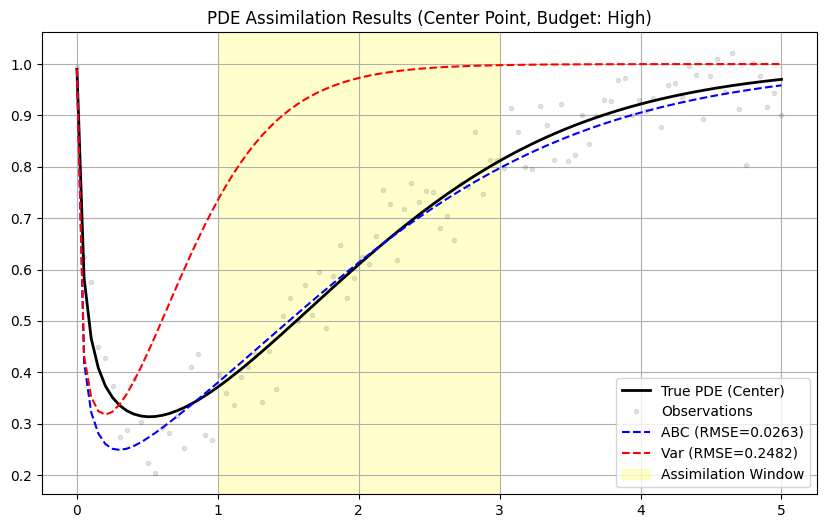
\includegraphics[width=0.6\textwidth]{../presentation/pde_assimilation_results_center_budget_high.png}
\end{frame}

% --- Zadanie 6 ---
\begin{frame}{Zadanie 6 — PINN}
\begin{itemize}
  \item PINN: trenowana z loss = data + physics; techniki: residualy, warm-up \(\lambda_{phy}\), schedulery.
  \item Wynik (ulepszone): MAE 0.0312, RMSE 0.0583 — znacząca redukcja błędu względem baseline.
\end{itemize}
\vspace{0.6em}
\centering
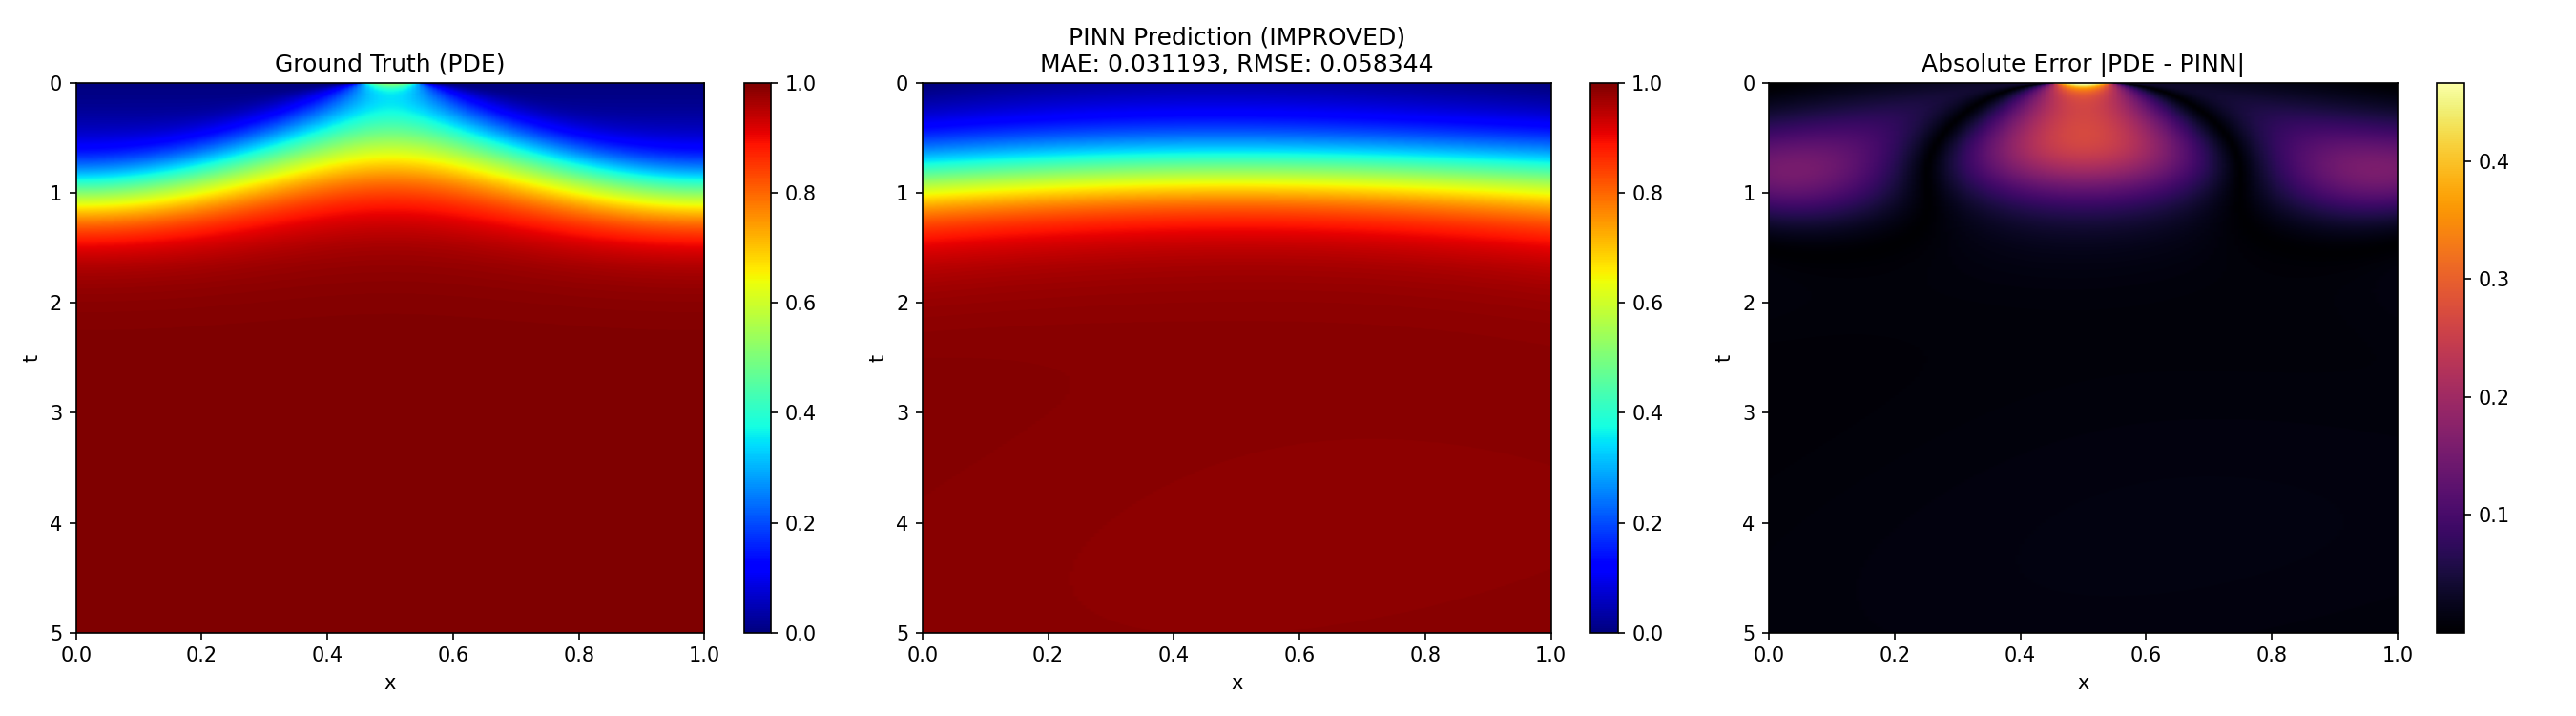
\includegraphics[width=0.7\textwidth]{../zad6/results/pinn_results_heatmap_improved.png}
\end{frame}

% --- Zadanie 7 ---
\begin{frame}{Zadanie 7 — Supermodel i SuperNet}
\begin{itemize}
  \item Supermodel ODE (ensemble + nudging) redukuje błąd (RMSE: 0.0451 vs single 0.1116).
  \item SuperNet PINN (ensemble PINN + coupling) osiąga najlepsze wyniki: MAE 0.0172, RMSE 0.0178.
\end{itemize}
\vspace{0.6em}
\centering
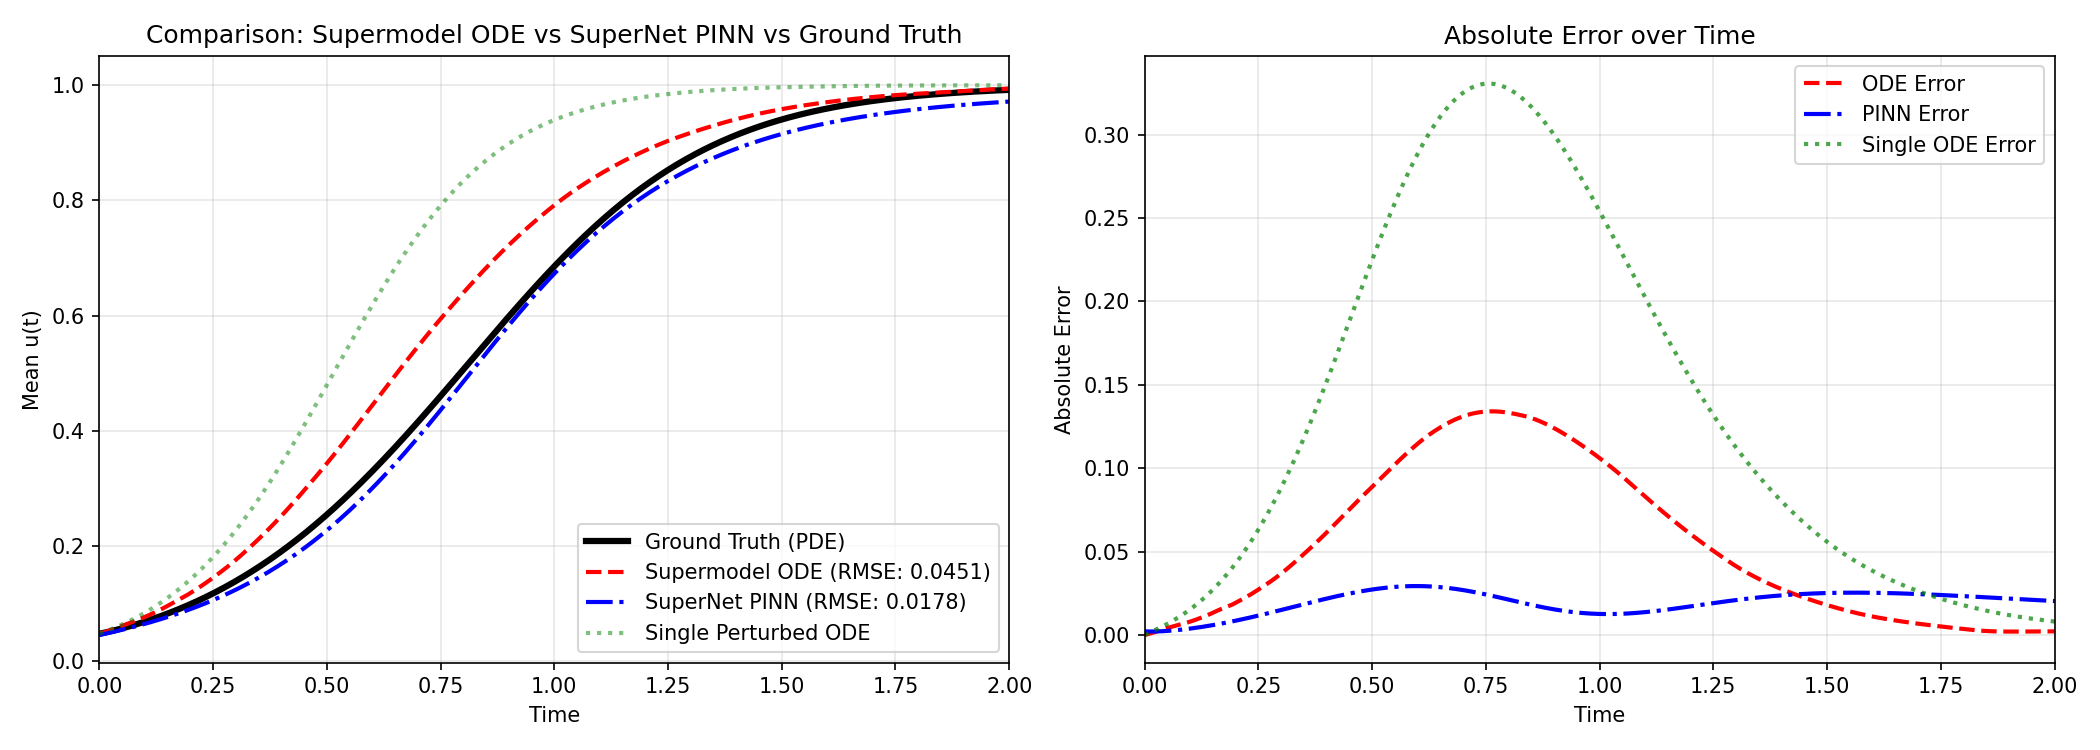
\includegraphics[width=0.75\textwidth]{../zad7/results/supermodel_vs_supernet_improved.png}
\end{frame}

\end{document}
